\documentclass[10pt,hyperref={CJKbookmarks=true},xcolor=dvipsnames,aspectratio=169]{beamer}
\usetheme[navigation]{UMONS}
\usepackage[utf8]{inputenc}
\usepackage{verbatim}
\usepackage{ctex}

\title[国际经济学]{国际经济学}
\subtitle{贸易政策的政治经济分析}
\author{鲁晓东}
\institute[]{%
	岭南学院\hspace{2em}中山大学
	\\[4ex]
	
\includegraphics[height=8ex]{fig/lingnanlogo}\hspace{2em}%
	
\includegraphics[height=8.5ex]{fig/sysu}
}
%------------section前展示一页----------
\AtBeginSection[] {     
	\begin{frame}        
	\tableofcontents[currentsection,hideallsubsections]    
\end{frame} 
}

%-------------subsection也展示一下----------
\AtBeginSubsection[]{

\frame<beamer>{ 
	
	\frametitle{Outline}   
	
	\tableofcontents[currentsection,currentsubsection] 
	
}

}
%---------------------------

%-----------一段一闪现-------
%\beamerdefaultoverlayspecification{<+->}
%这个功能基本不用

\begin{document}
\maketitle


\begin{frame}
\frametitle{提纲}
\tableofcontents
\end{frame}				%生成提纲页

%-----------正文开始----------------------

%\beamerdefaultoverlayspecification{<+->}
\section{Motivation}

\begin{frame}{1999中国入世谈判的临门一脚}
	\centering 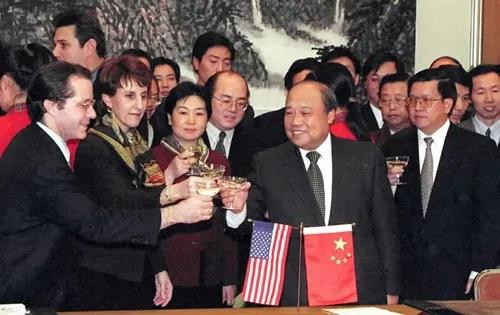
\includegraphics[scale=0.7]{fig/politic/wto}\\
“龙永图,你不要再递条子了。”\\

面对中国WTO首席谈判代表龙永图递上来的一个又一个\structure{条子},朱镕基断喝。1999年11月15日,中美谈判最后一天上午,这是中国加入WTO双边谈判最困难的时刻。\\
——摘自《那年入世谈判,我们经历了什么》,瞭望智库
\end{frame}

\section{支持自由贸易的观点}
\begin{frame}{Chapter 10 : Politics and Trade Policy}

\begin{itemize}
	\item Some additional arguments for Free Trade
	\item Arguments Against Free Trade
	\begin{itemize}
		\item National Welfare reasons 
		\item Income Distribution and Trade Policy
	\end{itemize}
	\item International Negotiations
	\begin{itemize}
		\item Some theory
		\item A short history of International Trade Agreements 
		\item Preferential Trade Arrangements
	\end{itemize}
\end{itemize}

\end{frame}

\begin{frame}{Some more arguments for Free Trade}

\begin{itemize}
\item Chap. 1-8: gains from trade
\item What else?
\begin{itemize}
	\item Stuff we sort of already talked about
	\item The rent seeking distortions
	\item Politics and corruption
\end{itemize}
\end{itemize}

\end{frame}

\begin{frame}{Stuff we already mentioned}

\begin{itemize}
\item Efficiency losses for small countries making tariffs
\item Economies of scale, trade barriers reduce market size 
\item Innovation, hard to pick winners
\item Gains from shifting production to more productive firms
\end{itemize}

\end{frame}

\begin{frame}{Efficiency losses of tariff}

\centering 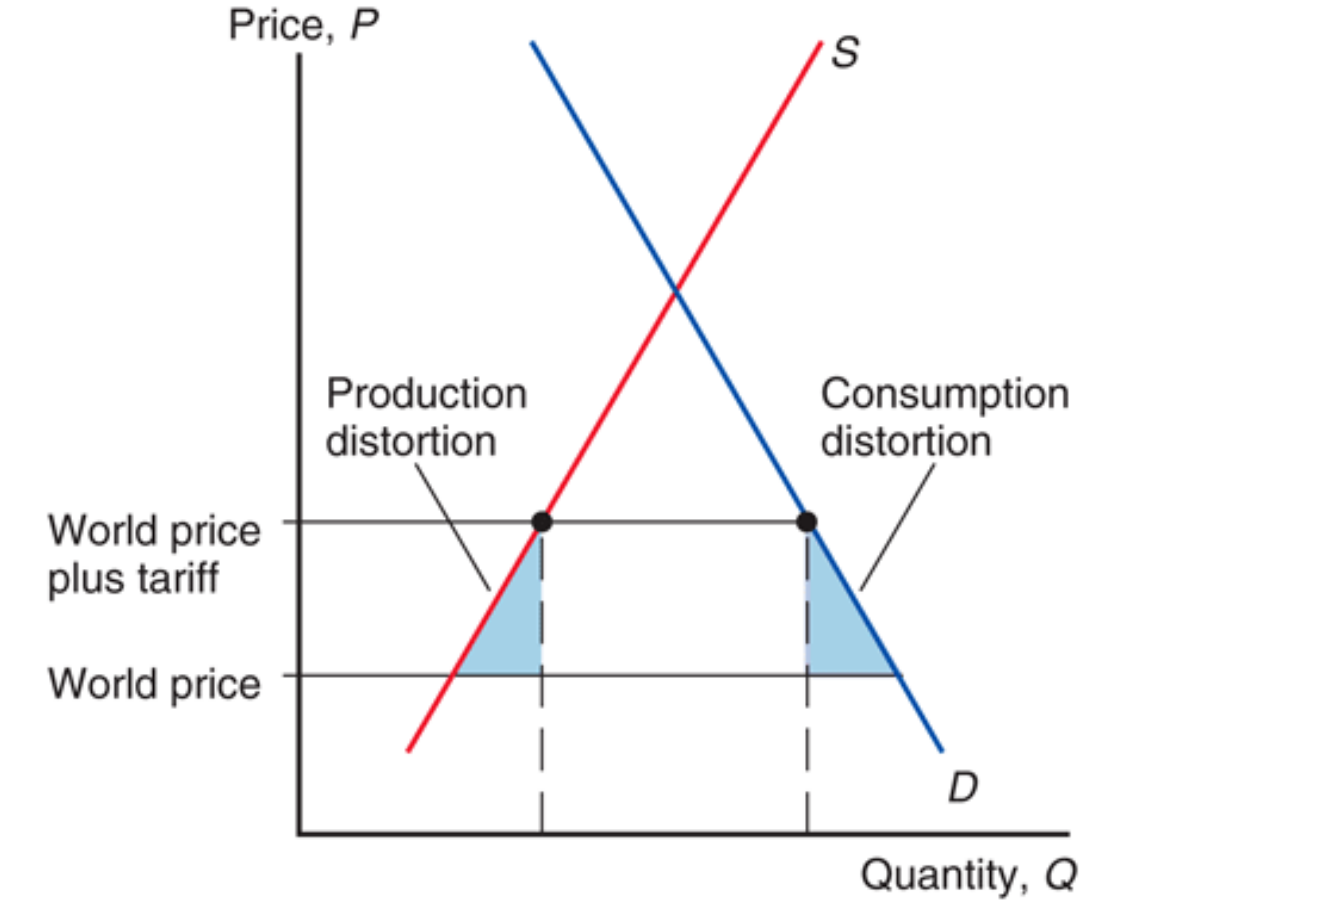
\includegraphics[scale=0.2]{fig/politic/tariff_distortion.png}

\end{frame}

\begin{frame}{Rent seeking distortions}

\begin{itemize}
\item Suppose we have import quotas
\item How to allocate?
\item Allocation system distorts production
\begin{itemize}
\item Example 1: India inport licenses based on capacity, build unneeded capacity
\item Example 2: US Tuna import licenses first come first serve, warehouse in December, big rush on Jan. 1st
\end{itemize}
\item Side note: License Raj in India
\end{itemize}

\end{frame}

\begin{frame}{Political Process and Corruption}

\begin{itemize}
\item Trade policy good in theory
\item Politics is messy
\begin{itemize}
\item Even good intentioned policies likely to be captured by special interest groups
\item Might cause even bigger distortions
\item Here free trade is a second best 
\end{itemize} 
\item Similar argument to why one should follow unjust laws
\end{itemize}

\end{frame}

\begin{frame}{Size of gains from free trade}
\begin{itemize}
\item Tariffs are already low, further gains small
\end{itemize}
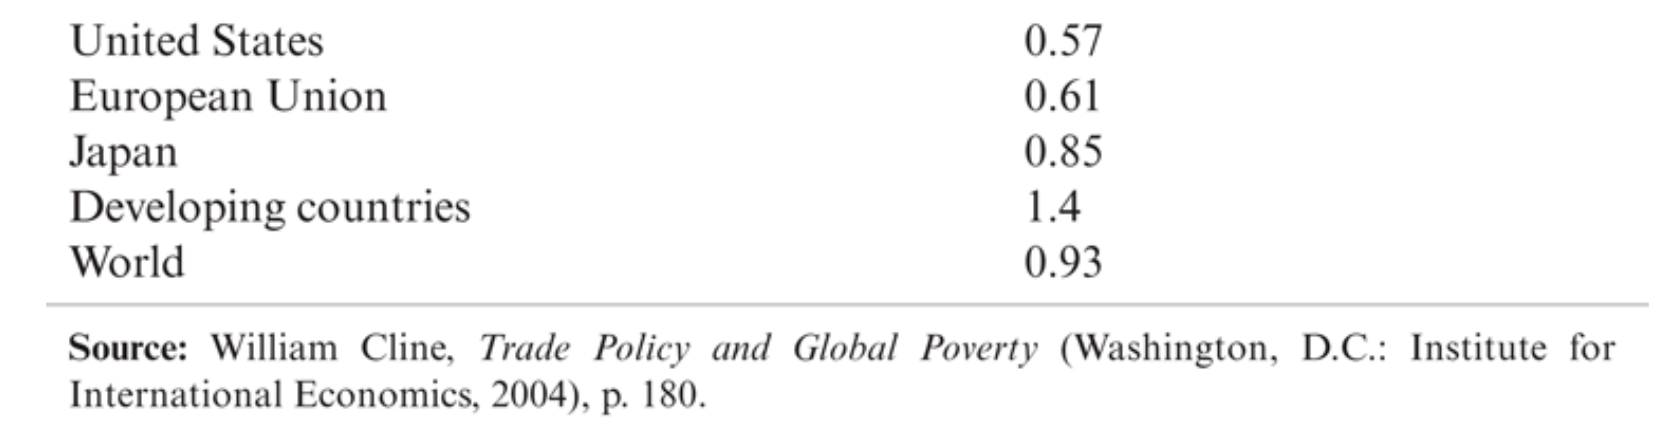
\includegraphics[scale=0.25]{fig/politic/trade_gains.png}
\end{frame}

\begin{frame}{Size of gains from trade}
\begin{itemize}
\item Research frontier: Gains from trade too small!
\begin{itemize}
\item We have arguments that countries gain from trade
\item Recently theory models have been estimable
\end{itemize}
\item Important new paper: Gains from trade in most models are the same
\begin{itemize}
\item Arkolakis, Costinot, Rodriguez, American Economic Review, 2012
\item United States going from autarchy to free trade welfare gains 0.7-1.4\% 
\item Compare this to estimates of gains from migration\dots
\end{itemize}
\end{itemize}

	\begin{block}{问题}
		So far, 我们已经学过三种stuff的跨国流动,分别是什么?基于哪种stuff的贸易自由化的边际收益最大?
	\end{block}
\end{frame}


\begin{frame}{Gains from trade vs migration}
\centering 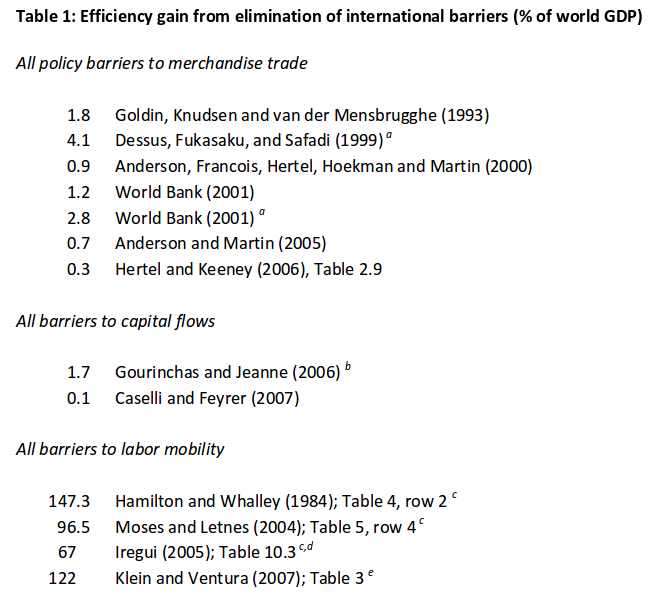
\includegraphics[scale=0.25]{fig/politic/gains_to_migration.png}

{\tiny Source: Clemens, Michael, ``Economics and Emigration: Trillion Dollar Bills on the Sidewalk?'', Journal of Economic Perspectives, 2011}
\end{frame}

\begin{frame}{小结}
\begin{itemize}
\item We have seen more arguments for free trade
\begin{itemize}
\item Classical gains from trade
\item Trade policy causes rent seeking distortions
\item Trade policy is often captured by special interests
\end{itemize}
\item \textbf{\textcolor{red}{Now we will focus on arguments against free trade}}
\begin{itemize}
\item The optimum tariff
\item Domestic market failure and trade policy
\end{itemize}
\end{itemize}
\end{frame}

\section{反对自由贸易的观点}
\begin{frame}{The optimum tariff}
\begin{itemize}
\item We saw that optimum tariff levels are always positive
\item Same argument can be used to justify optimum export tax!
\end{itemize}
\centering 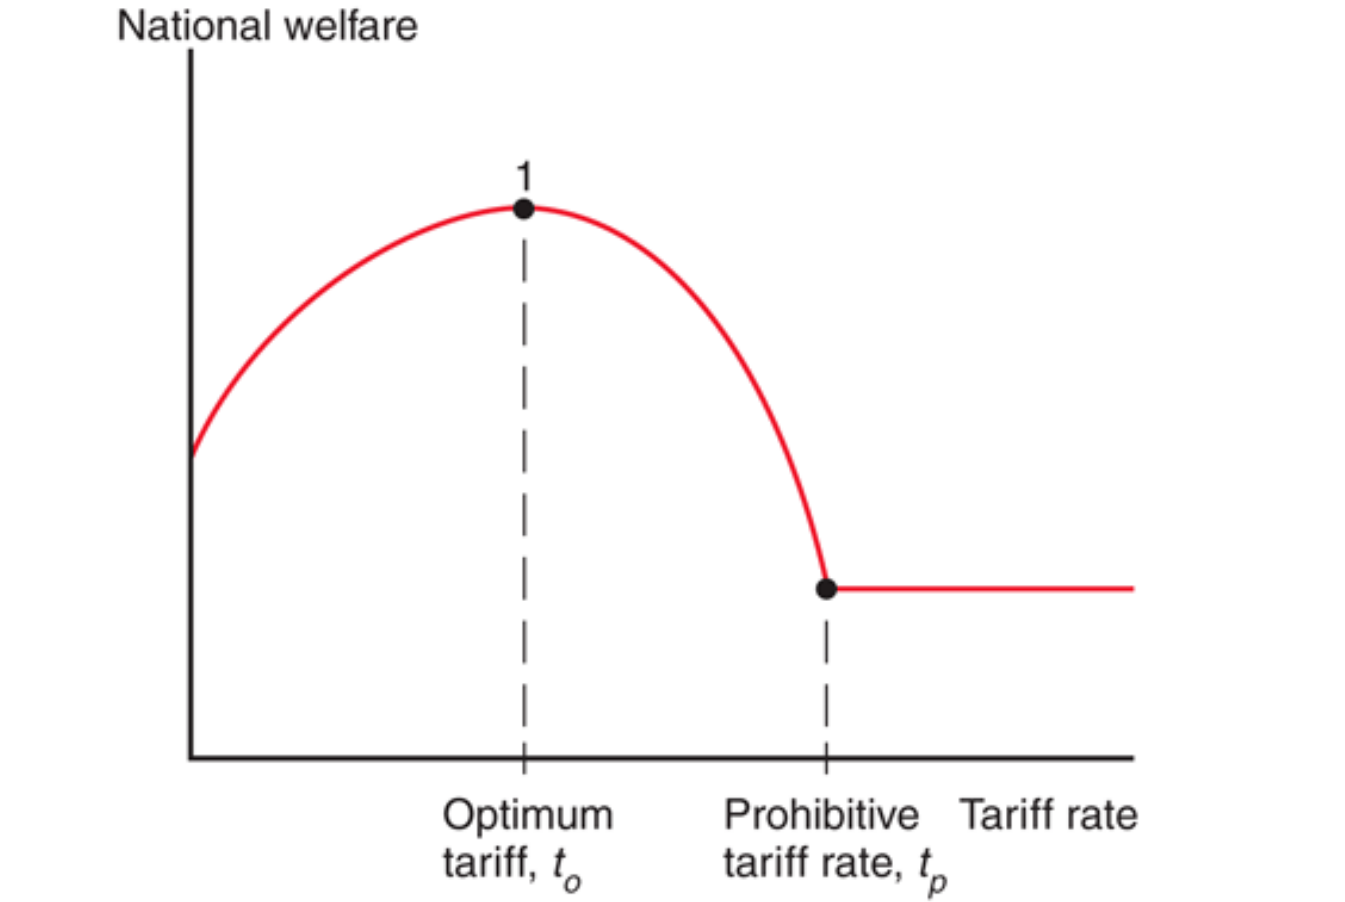
\includegraphics[scale=0.20]{fig/politic/optimum_tariff.png}
\end{frame}


\begin{frame}{The optimum tariff}
\begin{itemize}
\item Why do we rarely see export taxes?
\item Why are tariff levels currently so low?
\item Why don't large countries impose tariffs on small countries?
\end{itemize}
\end{frame}


\begin{frame}{The theory of the second best次优理论}
\begin{itemize}
\item Markets are great, but plenty of market failures
\begin{itemize}
\item Traffic is one example of an externality
\item Pollution is another
\item Typically things worse in developing countries
\end{itemize}
\item The best policy is usually to tax the externality
\item But if that isn't possible, maybe trade policy can help
\begin{itemize}
\item Suppose corruption makes it hard for new manufacturing firms to enter
\item Too little manufacturing
\item We could use trade policy to encourage entry into manufacturing
\end{itemize}
\item On the other hand
\begin{itemize}
\item It is hard to choose winners
\item Effects of second-best costly and hard to predict
\end{itemize}
\end{itemize}
\end{frame}

\begin{frame}{小结}
\begin{itemize}
\item We have seen more arguments for free trade
\begin{itemize}
\item Classical gains from trade
\item Trade policy causes rent seeking distortions
\item Trade policy is often captured by special interests
\end{itemize}
\item We have seen arguments against free trade
\begin{itemize}
\item The optimum tariff
\item Domestic market failure and trade policy
\end{itemize}
\item  \textbf{\textcolor{red}{\emph{Now we will talk about how trade policy is formed}}}
\end{itemize}
\end{frame}

\section{贸易政策的政治经济模型}
\frame{
\frametitle{Political Models of Trade Policy}
Models related to trade policy:
\begin{enumerate}
\item Median voter theorem中点选民模型
\item Collective action集体行动理论
\end{enumerate}
}
\subsection{Median voter theorem}
\frame{
\frametitle{Median Voter Theorem}
Do you still remember the \structure{Hotelling Model} in Microeconomics\\
Electoral competition can be modeled as:
\begin{itemize}
\item Two parties
\item Continuum of voters of size $N$
\item Line the voters up by their preferred tariff
\item A voter chooses the party closest to her preferred tariff
\item Parties take tariff positions to maximize support
\item Suppose that voters have a uniform distribution over preferred tariffs between $0$ and $T$
\end{itemize}
}

\frame{
\frametitle{Median Voter Theorem}
\begin{columns}
	\begin{column}{0.5\textwidth}
		\begin{itemize}
			\item Both parties choose the same, median voter supported trade policy 
			\item What if there are three parties?
			\item Median voter theorem predictions contrast with trade policy
			\begin{itemize}
				\item Typically trade policy helps one industry a lot
				\item Typically trade policy hurts everyone else a little
			\end{itemize}
		\end{itemize}
	\end{column}
	\begin{column}{0.5\textwidth}
		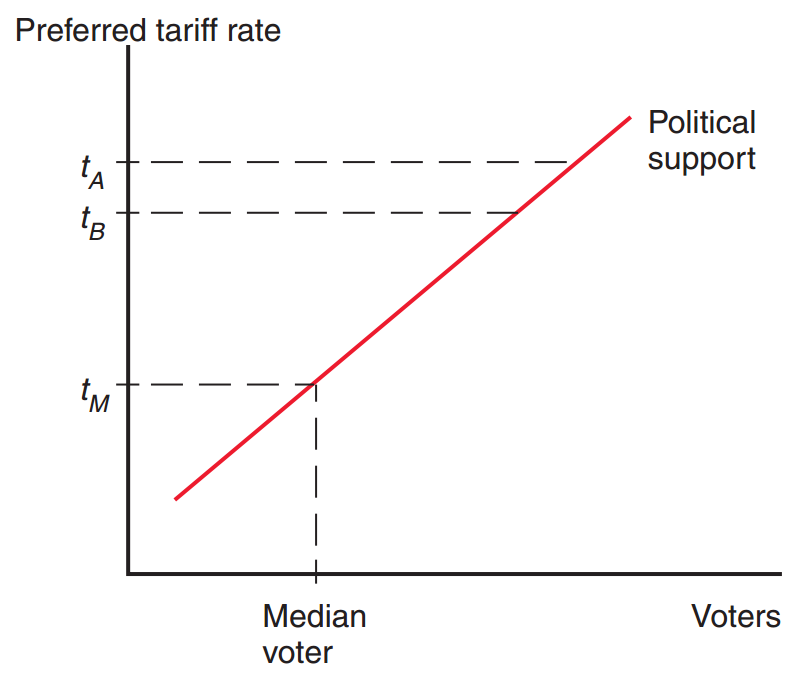
\includegraphics[scale=0.45]{fig/politic/medianvoter}
	\end{column}
\end{columns}

}
\subsection{Collective action}
\frame{
\frametitle{Collective Action}

\begin{itemize}
\item Trade policy is a \emph{public good}
\begin{itemize}
\item That is, it cannot be excluded
\end{itemize}
\item Nearly everyone in China hurt by beef import tariffs(12\%)
\item Suppose I write a letter to my representative
\begin{itemize}
\item The probability my letter is pivotal is small
\item The benefit I get from removing subsidies is (relatively) small
\item There is a small cost to sending a letter
\item I won't do it
\end{itemize}
\item Suppose I am a Chinese farmer
\begin{itemize}
\item The probability my letter is pivotal is larger (smaller group of potential writers)
\item The benefit I get from keeping tariff is much larger
\item There is a small cost to sending a letter 
\item I do it
\end{itemize}
\item Result: \structure{All the letters from farmers}
\end{itemize}
}

\frame{
\frametitle{Punchline: Collective action}
\begin{itemize}
\item Policies with large aggregate loss but small individual loss are difficult to change
\item Small groups with concentrated losses are more willing to pay effort fixed cost 
\item 会哭的孩子有奶吃
\end{itemize}
}

\frame{
\frametitle{Real Politics}
\begin{itemize}
\item Politicians win elections partly because: 
\begin{enumerate} 
\item they advocate popular policies (median voter theorem)
\item they have funds to run campaigns (collective action)
\end{enumerate}
\item We indeed get the trade policy in well-organized groups with concentrated gains(能够克服集体行动困难) 
\end{itemize}
}

\frame{
\frametitle{Which Industries are Protected?}
\begin{itemize}
\item Agriculture 
\begin{itemize}
\item Small but politically vocal labor force in the US
\item Japan has 1000\% tariff on rice imports!
\end{itemize}
\item Textiles (USA, about 14 \$ billion)
\begin{itemize}
\item Declining in importance thanks to WTO
\item Billions of dollars in US welfare loss due to protection:
\end{itemize}
\end{itemize}
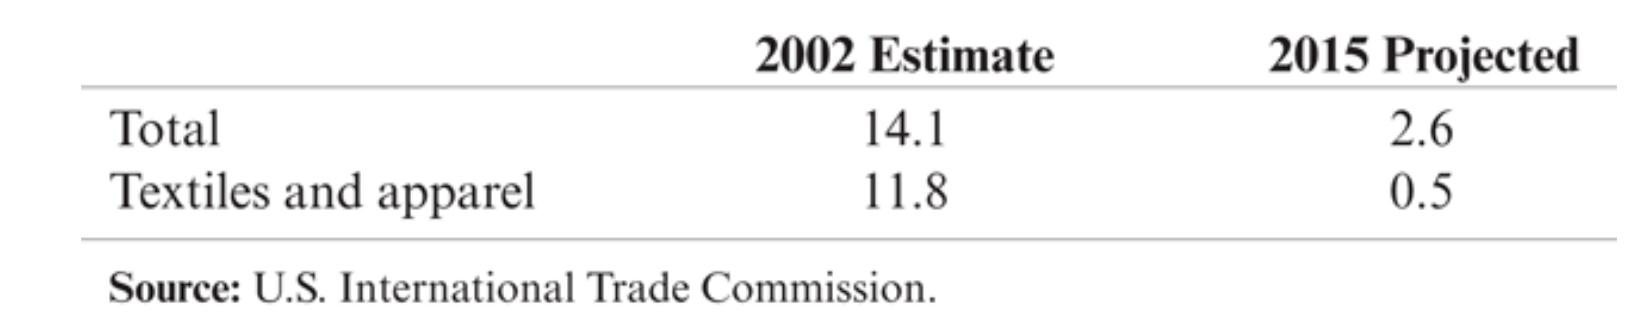
\includegraphics[scale=0.20]{fig/politic/textiles_welfare.png}
}



\section{综合案例:美国的糖配额}

\begin{frame}{Example: U.S. Sugar Quota}

\begin{itemize}
\item U.S. guarantees sugar producers a “break even” price保本价 on sugar production 
\item The USDA will buy any amount of sugar at this price 
\item Even at this relatively high price, domestic demand exceeds domestic
supply of sugar, so the US imports sugar 
\item In order to maintain this higher price, the US imposes a sugar quota
and lets foreign governments administer the quota and retain the quota
rents 
\item Over the past 25 years, this higher price has been on average twice
the world market price of sugar
\end{itemize}
\end{frame}

\begin{frame}{Welfare Effects of U.S. Sugar Quota}






\begin{columns}[onlytextwidth]
\begin{column}{0.4\textwidth}
\begin{itemize}
\item CS loss ($a+b+c+d$): \$884M 
\item PS gain ($a$): \$272M 
\item Distortion in: 

\begin{itemize}
\item Production ($b$): \$68M 
\item Consumption ($d$): \$91M 
\end{itemize}
\item Quota rents ($c$): \$453M 
\item Net surplus loss ($b+c+d$): \$612M
\end{itemize}

\end{column}
\begin{column}{0.6\textwidth}
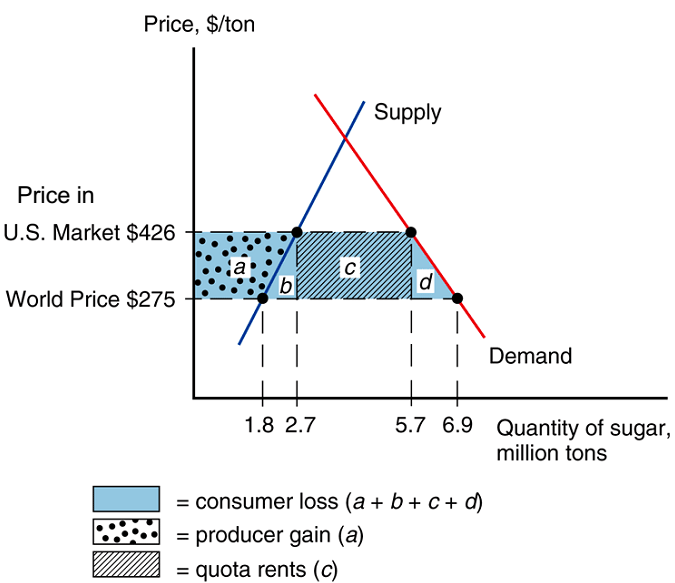
\includegraphics[width=0.8\columnwidth]{fig/politic/lec07-13}
\end{column}
\end{columns}

\end{frame}

\begin{frame}{Winners and Losers}

\begin{itemize}
\item US sugar industry employs 6,500 workers 

\begin{itemize}
\item PS gains represent \$42K per worker 
\end{itemize}
\item The quota does increase employment in the sugar industry: employment
would be 32\% lower without quota 

\begin{itemize}
\item This represents a cost to U.S. consumers of \$432K per job saved!
 Considering employment losses from the quota in sugarusing industries,
then net employment effect of quota is negative and cost per job saved
goes up to \$826K 
\end{itemize}
\item On average, each US consumer pays an extra \$3 (per year) from the
higher US sugar price (\$11 per family) 
\item Who do you think benefits?
\end{itemize}
\end{frame}

\begin{frame}{Winners and Losers (cted.)}

\begin{itemize}
\item The US sugar industry is very concentrated geographically (in Florida)
and very well organized 
\item US sugar sales represent 1\% of US farm receipts and 0.5\% of US farm
employment 
\item US sugar lobby contributions represent 17\% of campaign contributions
from agricultural sector 
\item The Fanjul brothers who own Flo-Sun (the biggest US sugar cane growing
and refining company) gave \$1M in political contributions in each
of the 2000 and 2004 election cycles
\end{itemize}
\end{frame}

\begin{frame}{Two Winners}


\begin{figure}


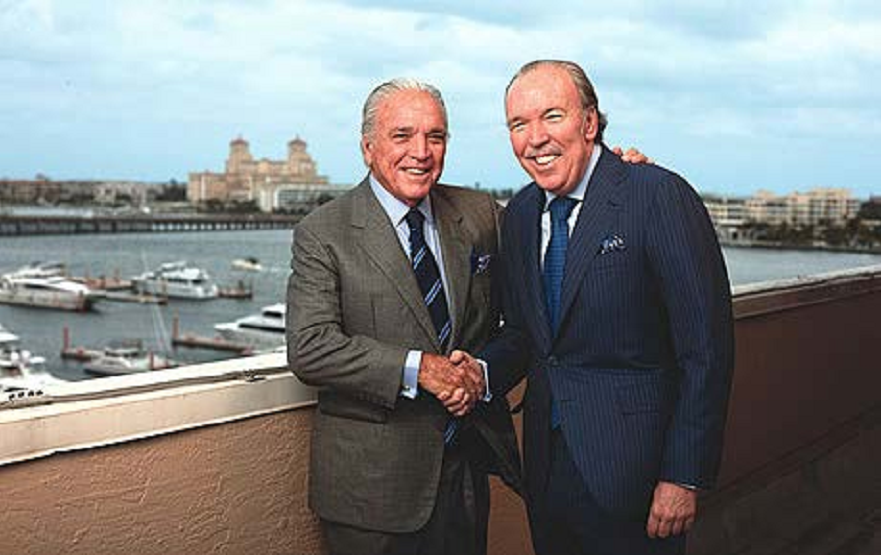
\includegraphics[scale=0.4]{fig/politic/lec07-14}

\end{figure}

\end{frame}

\begin{frame}{Political Economy of Sugar Quotas}

\begin{itemize}
\item In 1996, a congressional amendment was introduced to phase out the
US sugar quota (and price support program) 
\item The amendment was defeated by 217-209 in the house of representatives 
\item Five co-sponsors of the bill switched their support against their
own amendment in the final vote 
\item Within days of the vote, each received an average of \$11,000 from
the US sugar lobby
\end{itemize}
\end{frame}

\begin{frame}{总结}
\begin{itemize}
	\item We have seen more arguments for free trade
	\begin{itemize}
		\item Classical gains from trade
		\item Trade policy causes rent seeking distortions
		\item Trade policy is often captured by special interests
	\end{itemize}
	\item We have seen arguments against free trade
	\begin{itemize}
		\item The optimum tariff
		\item Domestic market failure and trade policy
	\end{itemize}
	\item We have talk about how trade policy is formed
	\begin{itemize}
		\item Median voter
		\item Collective action
	\end{itemize}
\end{itemize}
\end{frame}


\end{document}